% Provenance (never printed): cycle 3 / 6e "La planete Terre" (water in the
% ground, groundwater, springs and wells; resource); see
% sources/book1/PROVENANCE.md. Book 1, grade 6, chapter 5.
% Vocabulary guard: "sediment" not before g7.4; the water cycle is recalled
% from the physics book (prose only).
\chapter{El agua bajo tierra}\label{ch:g6:water-underground}

Es un caluroso día de verano: los campos están secos y los arroyos llevan
poca agua. Y, sin embargo, al pie de una \omterm{def:g1:landscapes-around-us:landform}{colina} sigue brotando agua del
suelo, fría y transparente, como durante todo el invierno, y llena una
poza. Hace semanas que no llueve. ¿De dónde viene esta agua, y cómo sale de
la \omterm{def:g3:stones-pebbles-sand:rock}{roca}?

\begin{omfigure}
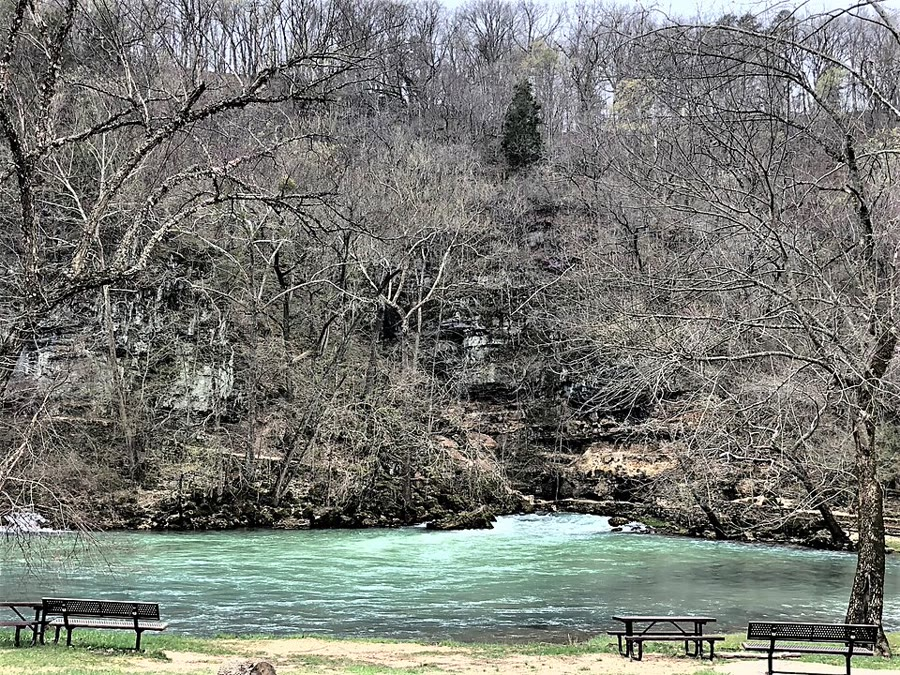
\includegraphics[width=0.72\linewidth]{images/book1/g6-big-spring.jpg}

{\small Un \omterm{def:g6:water-underground:spring}{manantial} brota al pie de un escarpe rocoso y llena una poza:
Big Spring, Misuri (Estados Unidos). (Foto: Johnston9494, CC BY-SA 4.0, vía
Wikimedia Commons.)}
% ledger: commons:big-spring
\end{omfigure}

\begin{recall}
Casi toda el agua de la Tierra es \omterm{def:g2:water-on-earth:salt-fresh}{agua salada}; el \omterm{def:g2:water-on-earth:salt-fresh}{agua dulce} es una parte
pequeña, guardada sobre todo en forma de hielo y bajo tierra
(\cref{ch:g2:water-on-earth}). \omterm{def:g3:stones-pebbles-sand:rock}{Rocas} como la arenisca y la caliza están
hechas de granos o de conchas unidos entre sí, mientras que la arcilla y la
lutita están hechas de partículas muy finas
(\cref{ch:g6:rocks-and-minerals}). En el libro de física has seguido el
agua a lo largo del ciclo del agua: se evapora de los \omterm{def:g2:water-on-earth:ocean}{mares}, se condensa
en \omterm{def:g4:clouds-rain-snow:cloud}{nubes} y vuelve a caer en forma de \omterm{def:g4:clouds-rain-snow:precipitation}{lluvia} o de \omterm{def:g4:clouds-rain-snow:precipitation}{nieve}.
\end{recall}

\section{La lluvia se infiltra}

Cuando la \omterm{def:g4:clouds-rain-snow:precipitation}{lluvia} cae sobre la tierra, el agua puede seguir tres caminos.
Una parte se evapora y vuelve al aire. Otra parte corre por la superficie,
ladera abajo, hasta los arroyos y los \omterm{def:g1:landscapes-around-us:water}{ríos}: es la \emph{escorrentía}. El
resto se infiltra en el suelo.

\begin{definition}[Infiltración]\label{def:g6:water-underground:infiltration}
La \emph{infiltración}\index{infiltracion@infiltración} es la entrada del
agua de \omterm{def:g4:clouds-rain-snow:precipitation}{lluvia}, o de la \omterm{def:g4:clouds-rain-snow:precipitation}{nieve} fundida, en el suelo, a través de la tierra y
hacia abajo, hasta las \omterm{def:g3:stones-pebbles-sand:rock}{rocas}.
\end{definition}

La cantidad de agua que se infiltra depende del terreno. En una pendiente
empinada, en un suelo desnudo o duro, en una carretera o en un aparcamiento,
o cuando el suelo ya está empapado, casi toda el agua corre por la
superficie. En una pendiente suave, bajo la hierba y los árboles, en un
suelo arenoso, una parte mayor tiene tiempo de infiltrarse.

\begin{omfigure}
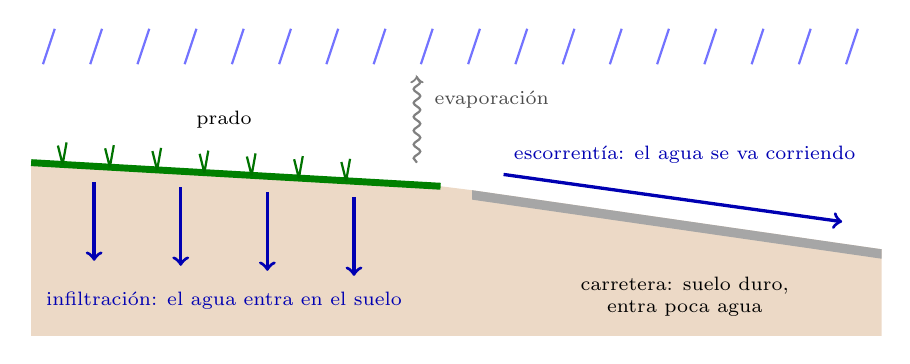
\begin{tikzpicture}[x=1cm, y=1cm]
  % rain
  \foreach \x in {0.3,0.9,...,10.5} \draw[blue!55, thick] (\x,3.9) -- (\x-0.15,3.45);
  % ground: field on the left (gentle), road and town on the right
  \fill[brown!30] (0,0) -- (0,2.2) -- (5.2,1.9) -- (5.6,1.85) -- (10.8,1.1) -- (10.8,0) -- cycle;
  \draw[green!50!black, line width=2.5pt] (0,2.2) -- (5.2,1.9);
  \fill[gray!70] (5.6,1.85) -- (10.8,1.1) -- (10.8,0.98) -- (5.6,1.73) -- cycle;
  \foreach \x in {0.4,1.0,...,4.6} \draw[green!45!black, thick] (\x,{2.2-0.058*\x}) -- ++(0.05,0.28) (\x,{2.2-0.058*\x}) -- ++(-0.06,0.24);
  % infiltration arrows in the field
  \foreach \x in {0.8,1.9,3.0,4.1} \draw[->, blue!70!black, very thick] (\x,{2.0-0.058*\x}) -- ++(0,-1.0);
  \node[font=\scriptsize, blue!70!black, align=center, fill=brown!30] at (2.45,0.45) {infiltración: el agua entra en el suelo};
  % run-off on the road
  \draw[->, blue!70!black, very thick] (6.0,2.05) -- (10.3,1.45);
  \node[font=\scriptsize, blue!70!black, align=center] at (8.3,2.3) {escorrentía: el agua se va corriendo};
  \node[font=\scriptsize, align=center] at (8.3,0.5) {carretera: suelo duro,\\ entra poca agua};
  \node[font=\scriptsize] at (2.45,2.75) {prado};
  % evaporation
  \draw[->, gray, thick, decorate, decoration={snake, amplitude=1.2pt, segment length=5pt}] (4.9,2.2) -- (4.9,3.3);
  \node[font=\scriptsize, gray!60!black, anchor=west] at (5.0,3.0) {evaporación};
\end{tikzpicture}

{\small Los tres caminos del agua de \omterm{def:g4:clouds-rain-snow:precipitation}{lluvia}. En el prado, buena parte se
infiltra; en la carretera, casi toda corre por la superficie.}
\end{omfigure}

\section{Rocas porosas y permeables}

Mira con una lupa un puñado de \omterm{def:g3:stones-pebbles-sand:sand}{arena} seca: entre los granos hay espacios
vacíos diminutos. Echa agua encima y el agua llena esos espacios. Muchas
\omterm{def:g3:stones-pebbles-sand:rock}{rocas} son así: están llenas de agujeritos entre sus granos, o de grietas
finas.

\begin{definition}[Porosidad]\label{def:g6:water-underground:porosity}
Los \emph{poros}\index{poro} de una \omterm{def:g3:stones-pebbles-sand:rock}{roca} son los espacios vacíos que hay
entre sus granos y en sus grietas. Una \omterm{def:g3:stones-pebbles-sand:rock}{roca} con poros es
\emph{porosa}\index{poroso}. Su \emph{porosidad}\index{porosidad} es la
parte de su volumen formada por poros, escrita como porcentaje.
\end{definition}

\begin{definition}[Permeabilidad]\label{def:g6:water-underground:permeability}
Una \omterm{def:g3:stones-pebbles-sand:rock}{roca} es \emph{permeable}\index{permeable} cuando el agua puede
atravesarla, porque sus \omterm{def:g6:water-underground:porosity}{poros} son lo bastante grandes y están conectados
entre sí. Es \emph{impermeable}\index{impermeable} cuando el agua no puede
atravesarla. La \emph{permeabilidad}\index{permeabilidad} es la facilidad
con que el agua atraviesa una \omterm{def:g3:stones-pebbles-sand:rock}{roca}.
\end{definition}

Las dos ideas no son iguales. La arcilla es muy \omterm{def:g6:water-underground:porosity}{porosa}: la mitad de su
volumen está formada por \omterm{def:g6:water-underground:porosity}{poros}. Pero sus \omterm{def:g6:water-underground:porosity}{poros} son tan diminutos que el agua
se queda pegada en ellos: la arcilla es \emph{\omterm{def:g6:water-underground:permeability}{impermeable}}. La \omterm{def:g3:stones-pebbles-sand:sand}{arena} tiene
menos \omterm{def:g6:water-underground:porosity}{poros} que la arcilla, pero son anchos y están conectados: la \omterm{def:g3:stones-pebbles-sand:sand}{arena} es
\emph{\omterm{def:g6:water-underground:permeability}{permeable}}. El granito sin grietas casi no tiene \omterm{def:g6:water-underground:porosity}{poros}.
% ledger: heath:porosity

\begin{omfigure}
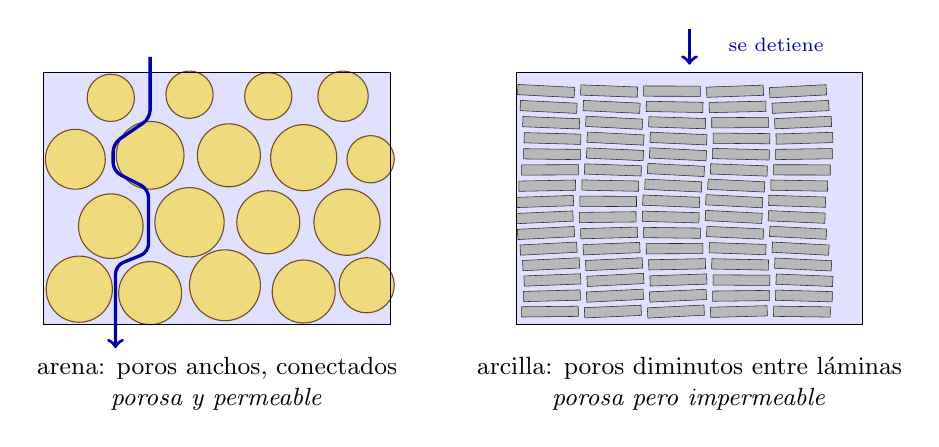
\begin{tikzpicture}
  % sand
  \begin{scope}
    \fill[blue!12] (0,0) rectangle (4.4,3.2);
    \foreach \x/\y/\r in {0.45/0.45/0.42, 1.35/0.4/0.4, 2.3/0.5/0.45, 3.3/0.42/0.4, 4.1/0.5/0.35,
                         0.85/1.25/0.41, 1.85/1.3/0.44, 2.85/1.3/0.4, 3.85/1.3/0.42,
                         0.4/2.1/0.38, 1.35/2.15/0.43, 2.35/2.15/0.4, 3.3/2.12/0.42, 4.15/2.1/0.3,
                         0.85/2.88/0.3, 1.85/2.92/0.3, 2.85/2.9/0.3, 3.8/2.9/0.32}
      \fill[yellow!55!brown!60, draw=brown!60!black] (\x,\y) circle (\r);
    \draw (0,0) rectangle (4.4,3.2);
    \draw[->, blue!70!black, very thick, rounded corners=3pt] (1.35,3.4) -- (1.35,2.62) -- (0.88,2.3) -- (0.88,1.95) -- (1.33,1.72) -- (1.33,0.92) -- (0.91,0.75) -- (0.91,-0.3);
    \node[font=\small, align=center] at (2.2,-0.75) {arena: poros anchos, conectados\\ \emph{porosa y permeable}};
  \end{scope}
  % clay
  \begin{scope}[xshift=6.0cm]
    \fill[blue!12] (0,0) rectangle (4.4,3.2);
    \foreach \y in {0.1,0.3,...,3.0}
      \foreach \x in {0.05,0.85,...,3.7}
        \fill[gray!55, draw=gray!30!black, line width=0.2pt, rotate around={{3*sin(57*\x+91*\y)}:(\x+0.36,\y+0.06)}]
          ({\x+0.05*sin(200*\y)},\y) rectangle ++(0.72,0.13);
    \draw (0,0) rectangle (4.4,3.2);
    \draw[->, blue!70!black, very thick] (2.2,3.75) -- (2.2,3.3);
    \node[font=\scriptsize, blue!70!black] at (3.3,3.55) {se detiene};
    \node[font=\small, align=center] at (2.2,-0.75) {arcilla: poros diminutos entre láminas\\ \emph{porosa pero impermeable}};
  \end{scope}
\end{tikzpicture}

{\small Los \omterm{def:g6:water-underground:porosity}{poros} (en azul) entre los granos de una \omterm{def:g3:stones-pebbles-sand:sand}{arena} y entre las
láminas de una arcilla, muy ampliados. El agua encuentra un camino a través
de la \omterm{def:g3:stones-pebbles-sand:sand}{arena}; en la arcilla, se queda pegada.}
\end{omfigure}

La tabla da la \omterm{def:g6:water-underground:porosity}{porosidad} de algunos materiales y la parte del agua que sale
de ellos por sí sola cuando están llenos de agua. El resto se queda pegado
a los granos.

\begin{center}\small
\begin{tabular}{|l|c|c|}
\hline
\textbf{material} & \textbf{\omterm{def:g6:water-underground:porosity}{porosidad} (\%)} & \textbf{agua que sale (\%)} \\
\hline
suelo & 55 & 40 \\
arcilla & 50 & 2 \\
\omterm{def:g3:stones-pebbles-sand:sand}{arena} & 25 & 22 \\
\omterm{def:g3:stones-pebbles-sand:pebble}{grava} & 20 & 19 \\
caliza & 20 & 18 \\
arenisca & 11 & 6 \\
granito & 0.1 & 0.09 \\
\hline
\end{tabular}
\end{center}
% ledger: heath:porosity

\begin{method}[¿Cuánta agua contiene una roca?]\label{met:g6:water-underground:volume}
\begin{enumerate}
  \item Halla el volumen de la \omterm{def:g3:stones-pebbles-sand:rock}{roca} (para un bloque: largo $\times$ ancho
        $\times$ alto).
  \item Multiplica por la \omterm{def:g6:water-underground:porosity}{porosidad} y divide entre 100: es el volumen de los
        \omterm{def:g6:water-underground:porosity}{poros}, y por tanto el agua que contiene la \omterm{def:g3:stones-pebbles-sand:rock}{roca} cuando está llena.
  \item Para el agua que sale, usa el segundo porcentaje de la misma
        manera. (1~metro cúbico son 1000~litros.)
\end{enumerate}
\end{method}

\begin{example}[Un metro cúbico de arena]\label{ex:g6:water-underground:sand}
Un metro cúbico de \omterm{def:g3:stones-pebbles-sand:sand}{arena}, lleno de agua, contiene en sus \omterm{def:g6:water-underground:porosity}{poros}
$1000 \times 25 \div 100 =
250$~litros de agua. De ellos, $1000 \times 22 \div 100 = 220$
litros salen por sí solos; 30~litros se quedan pegados a los granos. Un
metro cúbico de arcilla contiene el doble de agua, 500~litros, pero solo
salen 20~litros.
% ledger: heath:porosity
\end{example}

\begin{inthelab}[¿Arena o arcilla? (en clase, con el profesor)]
Dos macetas con un agujero en el fondo están colocadas sobre dos vasos. Una
se llena de \omterm{def:g3:stones-pebbles-sand:sand}{arena} seca, y la otra, de tierra arcillosa seca bien apretada.
El profesor echa el mismo vaso de agua en cada una, al mismo tiempo. A
través de la \omterm{def:g3:stones-pebbles-sand:sand}{arena}, el agua pronto gotea en el vaso de abajo. Sobre la
arcilla, el agua se queda arriba formando un charco y solo pasan unas pocas
gotas, despacio: la \omterm{def:g3:stones-pebbles-sand:sand}{arena} es \omterm{def:g6:water-underground:permeability}{permeable}, y la arcilla, no.
\end{inthelab}

\section{El agua subterránea y el nivel freático}

Cava un hoyo en la \omterm{def:g3:stones-pebbles-sand:sand}{arena} de una playa, a unos pasos del \omterm{def:g2:water-on-earth:ocean}{mar}: al cabo de un
rato, aparece agua en el fondo del hoyo. Has llegado al lugar donde todos
los \omterm{def:g6:water-underground:porosity}{poros} de la \omterm{def:g3:stones-pebbles-sand:sand}{arena} están llenos de agua.
% ledger: wss:aquifer

\begin{definition}[Agua subterránea]\label{def:g6:water-underground:groundwater}
El \emph{agua subterránea}\index{agua subterranea@agua subterránea} es el
agua que hay bajo tierra, llenando los \omterm{def:g6:water-underground:porosity}{poros} y las grietas del suelo y de
las \omterm{def:g3:stones-pebbles-sand:rock}{rocas}.
\end{definition}

\begin{definition}[Nivel freático]\label{def:g6:water-underground:water-table}
Por debajo de cierta profundidad, todos los \omterm{def:g6:water-underground:porosity}{poros} de la \omterm{def:g3:stones-pebbles-sand:rock}{roca} están llenos
de agua. El \emph{nivel freático}\index{nivel freatico@nivel freático} es
el techo de esta zona llena de agua. Por encima de él, los \omterm{def:g6:water-underground:porosity}{poros} contienen
aire y un poco de agua; por debajo, están llenos de agua.
% ledger: wss:aquifer
\end{definition}

El \omterm{def:g6:water-underground:water-table}{nivel freático} no es plano. Sigue la forma del terreno, pero de manera
más suave: más alto bajo las \omterm{def:g1:landscapes-around-us:landform}{colinas} y más bajo bajo los \omterm{def:g1:landscapes-around-us:landform}{valles}. También
sube y baja con las estaciones. Después de una estación lluviosa, la \omterm{def:g4:clouds-rain-snow:precipitation}{lluvia}
que se ha infiltrado lo hace subir; después de una larga estación seca, el
agua se va despacio hacia los \omterm{def:g6:water-underground:spring}{manantiales} y los \omterm{def:g1:landscapes-around-us:water}{ríos}, y el \omterm{def:g6:water-underground:water-table}{nivel freático}
baja.

El \omterm{def:g6:water-underground:groundwater}{agua subterránea} es una gran reserva de \omterm{def:g2:water-on-earth:salt-fresh}{agua dulce}. De toda el \omterm{def:g2:water-on-earth:salt-fresh}{agua
dulce} de la Tierra, alrededor del 69~\% es hielo y \omterm{def:g4:clouds-rain-snow:precipitation}{nieve} permanente, y
alrededor del 30~\% es \omterm{def:g6:water-underground:groundwater}{agua subterránea}; el \omterm{def:g2:water-on-earth:salt-fresh}{agua dulce} de todos los \omterm{def:g1:landscapes-around-us:water}{lagos}
solo supone alrededor de la cuarta parte del uno por ciento. El \omterm{def:g6:water-underground:groundwater}{agua
subterránea} es más de cien veces más abundante que el \omterm{def:g2:water-on-earth:salt-fresh}{agua dulce} de los
\omterm{def:g1:landscapes-around-us:water}{lagos}.
% ledger: wss:fresh-shares

\begin{omfigure}
\begin{tikzpicture}
  \begin{axis}[xbar, width=0.8\linewidth, height=3.9cm, bar width=8pt,
      xmin=0, xmax=85, ymin=-0.6, ymax=4.6, y dir=reverse,
      ytick={0,...,4}, yticklabels={{hielo y nieve permanentes},{agua subterránea},{hielo del suelo y permafrost},{lagos},{todo lo demás}},
      xlabel={porcentaje de toda el agua dulce de la Tierra},
      axis x line=bottom, axis y line=left, axis line style={-},
      tick label style={font=\scriptsize}, label style={font=\small},
      nodes near coords, nodes near coords style={font=\scriptsize, anchor=west},
      point meta=explicit symbolic, enlarge y limits=false, clip=false]
    \addplot[fill=blue!35, draw=blue!60!black] table[x=pct, y=idx, meta=pct] {figdata/out/grade-6-water_table-fresh.dat};
  \end{axis}
\end{tikzpicture}

{\small Dónde está el \omterm{def:g2:water-on-earth:salt-fresh}{agua dulce} de la Tierra. Las barras de los \omterm{def:g1:landscapes-around-us:water}{lagos} y de
todo lo demás (los \omterm{def:g1:landscapes-around-us:water}{ríos}, el aire, el suelo, los pantanos, los seres vivos)
son demasiado cortas para verlas.}
% ledger: wss:fresh-shares (figdata/grade-6/water_table.py, part fresh)
\end{omfigure}

\section{Manantiales y pozos}

\begin{definition}[Manantial y pozo]\label{def:g6:water-underground:spring}
Un \emph{manantial}\index{manantial} es un lugar donde el \omterm{def:g6:water-underground:groundwater}{agua subterránea}
sale del suelo por sí sola, allí donde el \omterm{def:g6:water-underground:water-table}{nivel freático} se encuentra con
la superficie. Un \emph{pozo}\index{pozo} es un agujero excavado o perforado
hasta por debajo del \omterm{def:g6:water-underground:water-table}{nivel freático}, de modo que el \omterm{def:g6:water-underground:groundwater}{agua subterránea} llena
su fondo y se puede sacar.
\end{definition}

El corte de abajo atraviesa un \omterm{def:g1:landscapes-around-us:landform}{valle} de las Colinas de Varden, la región de
nuestros ejercicios. Las \omterm{def:g1:landscapes-around-us:landform}{colinas} son de creta, una caliza blanca, blanda,
\omterm{def:g6:water-underground:porosity}{porosa} y \omterm{def:g6:water-underground:permeability}{permeable}. Bajo la creta hay una capa de lutita, que es
\omterm{def:g6:water-underground:permeability}{impermeable}. La \omterm{def:g4:clouds-rain-snow:precipitation}{lluvia} se infiltra en la creta, llena sus \omterm{def:g6:water-underground:porosity}{poros} y se
detiene sobre la lutita.

\begin{omfigure}
\begin{tikzpicture}
\begin{axis}[omsection, width=0.95\linewidth, height=7.2cm,
    xmin=0, xmax=2.8, ymin=0, ymax=560,
    xlabel={distancia desde el extremo sur del corte (km)},
    ylabel={altura sobre el nivel del mar (m)},
    tick label style={font=\scriptsize}, label style={font=\small},
    clip mode=individual]
  \addplot[om lith={icsJurassic!40}{om limestone}, draw=black, line width=0.3pt, even odd rule] table {figdata/out/grade-6-water_table-unit-limestone.dat};
  \addplot[om lith={icsJurassic!15}{om shale}, draw=black, line width=0.3pt, even odd rule] table {figdata/out/grade-6-water_table-unit-shale.dat};
  \addplot[om lith={icsCretaceous!35}{om limestone}, draw=black, line width=0.3pt, even odd rule] table {figdata/out/grade-6-water_table-unit-chalk.dat};
  \addplot[lith alluvium, draw=black, line width=0.3pt, even odd rule] table {figdata/out/grade-6-water_table-unit-alluvium.dat};
  \addplot[black, thick] table {figdata/out/grade-6-water_table-ground.dat};
  \addplot[blue!75!black, very thick] table {figdata/out/grade-6-water_table-wet.dat};
  \addplot[blue!75!black, very thick, dashed] table {figdata/out/grade-6-water_table-dry.dat};
  % wells
  \addplot[fill=white, draw=black, line width=0.4pt] table {figdata/out/grade-6-water_table-well-rects.dat};
  % the well labels of figdata/out/grade-6-water_table-well-labels.dat, written here in Spanish
  \node[font=\scriptsize\bfseries, anchor=south east, fill=white, fill opacity=0.8, text opacity=1, inner sep=1pt] at (axis cs:1.45,401.3) {pozo~A};
  \node[font=\scriptsize\bfseries, anchor=south east, fill=white, fill opacity=0.8, text opacity=1, inner sep=1pt] at (axis cs:1.7,470.3) {pozo~B};
  % river and spring
  \addplot[only marks, mark=*, mark size=2.2pt, blue!75!black] table[x=s_km, y=z_m] {figdata/out/grade-6-water_table-points.dat};
  \node[font=\scriptsize, blue!70!black, anchor=south east] at (axis cs:0.215,140) {río};
  \node[font=\scriptsize, blue!70!black, anchor=east] at (axis cs:0.83,218) {manantial};
  \node[font=\scriptsize] at (axis cs:2.2,470) {creta (permeable)};
  \node[font=\scriptsize, fill=white, fill opacity=0.8, text opacity=1] at (axis cs:2.2,95) {lutita (impermeable)};
  \node[font=\scriptsize, fill=white, fill opacity=0.8, text opacity=1] at (axis cs:0.95,25) {caliza};
  \node[font=\scriptsize, blue!70!black, fill=white, fill opacity=0.8, text opacity=1, align=center] at (axis cs:2.15,250) {nivel freático:\\ tras la estación lluviosa (continuo)\\ tras la estación seca (discontinuo)};
\end{axis}
\end{tikzpicture}

{\small Un corte norte--sur de las Colinas de Varden, desde el \omterm{def:g1:landscapes-around-us:water}{río} hasta lo
alto de la ladera norte (alturas exageradas unas 2~veces). El agua
contenida en la creta se detiene sobre la lutita y sale en forma de
\omterm{def:g6:water-underground:spring}{manantial} donde la base de la creta corta la ladera. El \omterm{def:g6:water-underground:spring}{pozo}~A siempre
llega al agua; el \omterm{def:g6:water-underground:spring}{pozo}~B solo llega a ella después de la estación lluviosa.}
% (figdata/grade-6/water_table.py; region model figdata/shared/region.py)
\end{omfigure}

El \omterm{def:g6:water-underground:spring}{manantial} brota donde la base de la creta corta la ladera: el agua no
puede bajar a través de la lutita, así que corre por encima de ella y sale
en la pendiente. Mientras haya agua en la creta por encima de la lutita, el
\omterm{def:g6:water-underground:spring}{manantial} sigue manando, incluso en un verano seco: esa es la respuesta a
la pregunta del principio del capítulo.

Fíjate en los dos \omterm{def:g6:water-underground:spring}{pozos}. El \omterm{def:g6:water-underground:spring}{pozo}~A tiene 100~m de profundidad; su fondo está
por debajo del \omterm{def:g6:water-underground:water-table}{nivel freático} en todas las estaciones, así que siempre da
agua. El \omterm{def:g6:water-underground:spring}{pozo}~B es aún más profundo, de 105~m, pero se excavó más arriba en
la \omterm{def:g1:landscapes-around-us:landform}{colina}: su fondo está por debajo del \omterm{def:g6:water-underground:water-table}{nivel freático} después de la
estación lluviosa y por encima después de la estación seca. En verano, el
\omterm{def:g6:water-underground:spring}{pozo}~B se seca. Lo que importa no es la profundidad de un \omterm{def:g6:water-underground:spring}{pozo}, sino lo
mucho que su fondo baja por debajo del \omterm{def:g6:water-underground:water-table}{nivel freático} más bajo.
% (figdata/grade-6/water_table.py, part wells)

\begin{omfigure}
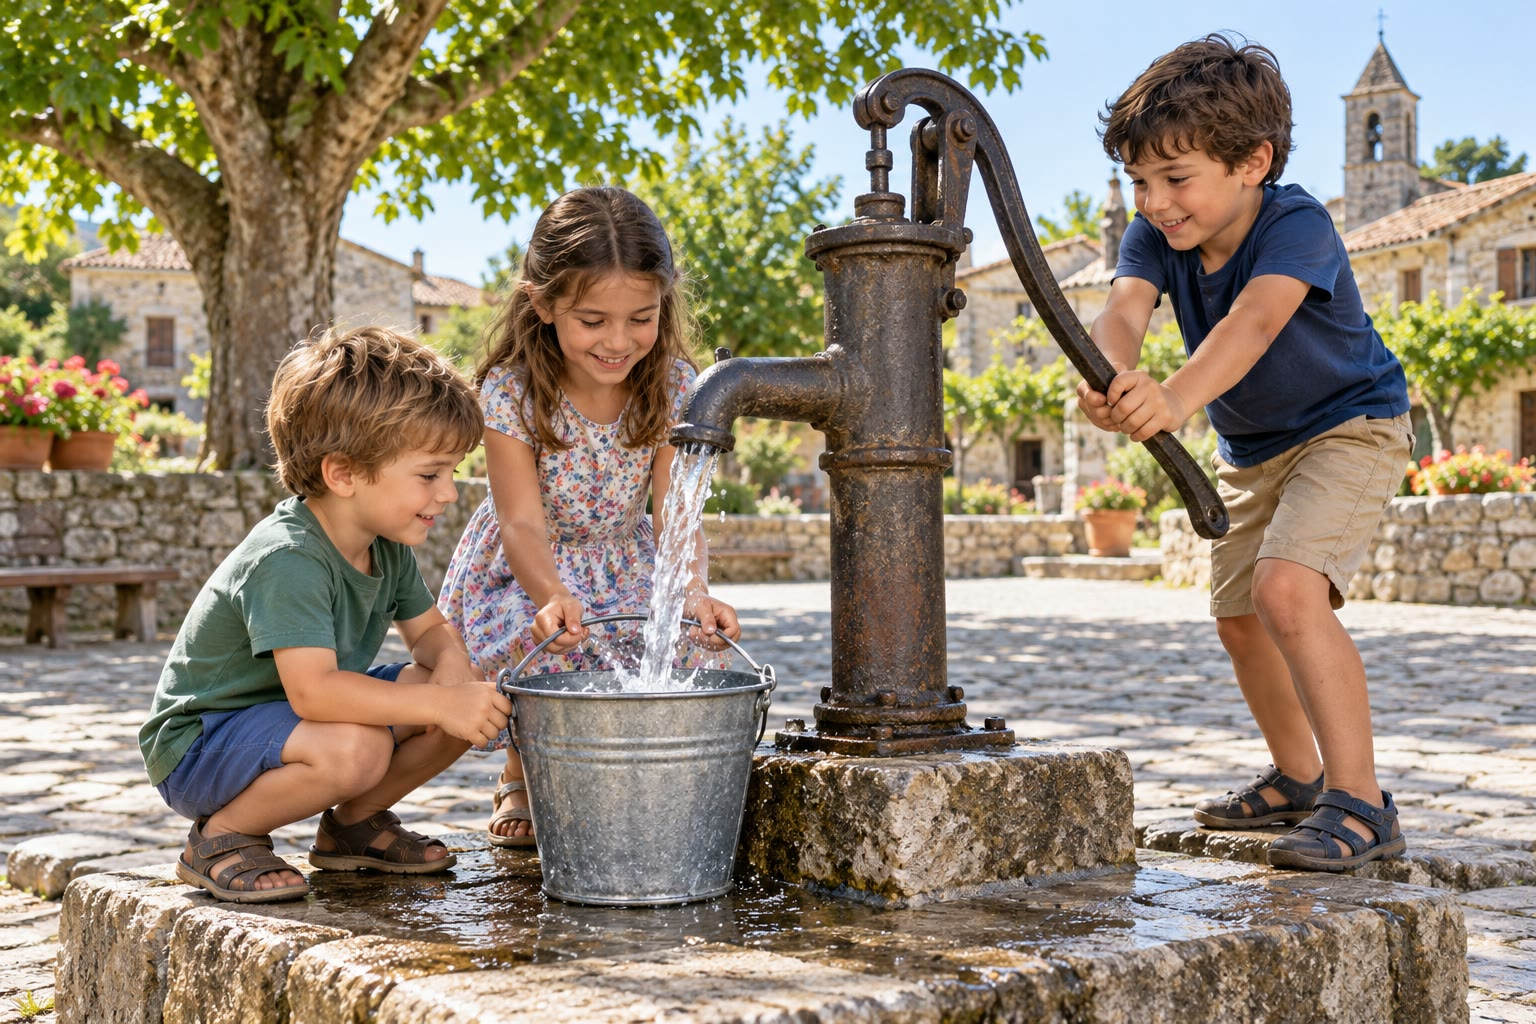
\includegraphics[width=0.6\linewidth]{images/book1/ai/g6-hand-pump.jpg}

{\small Unos niños llenan un cubo en la bomba de mano del \omterm{def:g6:water-underground:spring}{pozo} de un pueblo.
(Ilustración generada por IA.)}
\end{omfigure}

\begin{remark}[Un pozo puede secarse]\label{rem:g6:water-underground:pumping}
Bombear agua de un \omterm{def:g6:water-underground:spring}{pozo} hace bajar el \omterm{def:g6:water-underground:water-table}{nivel freático} a su alrededor. Si se
bombea el agua más deprisa de lo que la \omterm{def:g4:clouds-rain-snow:precipitation}{lluvia} vuelve a llenar la \omterm{def:g3:stones-pebbles-sand:rock}{roca}, el
\omterm{def:g6:water-underground:water-table}{nivel freático} baja y baja: el \omterm{def:g6:water-underground:spring}{pozo} da cada vez menos agua y puede secarse.
Dos vecinos que bombean de la misma \omterm{def:g3:stones-pebbles-sand:rock}{roca} comparten la misma agua: una bomba
puede secar el \omterm{def:g6:water-underground:spring}{pozo} del otro.
% ledger: wss:aquifer
\end{remark}

\section{Los acuíferos}

\begin{definition}[Acuífero]\label{def:g6:water-underground:aquifer}
Un \emph{acuífero}\index{acuifero@acuífero} es una capa de \omterm{def:g3:stones-pebbles-sand:rock}{roca} \omterm{def:g6:water-underground:porosity}{porosa} y
\omterm{def:g6:water-underground:permeability}{permeable}, llena de \omterm{def:g6:water-underground:groundwater}{agua subterránea}, que deja salir esa agua hacia los
\omterm{def:g6:water-underground:spring}{manantiales} y los \omterm{def:g6:water-underground:spring}{pozos}. La \omterm{def:g4:clouds-rain-snow:precipitation}{lluvia} que se infiltra vuelve a llenarla.
% ledger: wss:aquifer
\end{definition}

La creta de las Colinas de Varden es un \omterm{def:g6:water-underground:aquifer}{acuífero}: es \omterm{def:g6:water-underground:porosity}{porosa}, es \omterm{def:g6:water-underground:permeability}{permeable},
y las granjas de las \omterm{def:g1:landscapes-around-us:landform}{colinas} sacan de ella su agua. La lutita que hay
debajo no es un \omterm{def:g6:water-underground:aquifer}{acuífero}: el agua no puede atravesarla. Más abajo todavía,
bajo la lutita, hay una caliza y una arenisca, que también pueden contener
agua; para llegar a ella, hay que perforar un \omterm{def:g6:water-underground:spring}{pozo} que atraviese toda la
lutita.

El \omterm{def:g6:water-underground:groundwater}{agua subterránea} forma parte del ciclo del agua. La \omterm{def:g4:clouds-rain-snow:precipitation}{lluvia} se infiltra
en un \omterm{def:g6:water-underground:aquifer}{acuífero}; el \omterm{def:g6:water-underground:groundwater}{agua subterránea} corre despacio a través de los \omterm{def:g6:water-underground:porosity}{poros};
sale por los \omterm{def:g6:water-underground:spring}{manantiales} y hacia los \omterm{def:g1:landscapes-around-us:water}{ríos}, que la llevan al \omterm{def:g2:water-on-earth:ocean}{mar}; allí
se evapora y vuelve a caer en forma de \omterm{def:g4:clouds-rain-snow:precipitation}{lluvia}. Sacar agua de un \omterm{def:g6:water-underground:aquifer}{acuífero} es
como sacar agua de un depósito que la \omterm{def:g4:clouds-rain-snow:precipitation}{lluvia} llena despacio: solo dura si
no sacamos más de lo que la \omterm{def:g4:clouds-rain-snow:precipitation}{lluvia} devuelve.

\section{Mantener limpia el agua subterránea}

El agua que se infiltra en el suelo se filtra por el camino: las hojas, las
partículas de tierra y los pequeños animales quedan retenidos por el suelo
y la \omterm{def:g3:stones-pebbles-sand:rock}{roca}. Por eso el agua de un \omterm{def:g6:water-underground:spring}{manantial} o de un \omterm{def:g6:water-underground:spring}{pozo} suele parecer
cristalina. Pero las sustancias \emph{disueltas} en el agua no quedan
retenidas: bajan con ella hasta el \omterm{def:g6:water-underground:water-table}{nivel freático}.
% ledger: wss:gw-quality

El \omterm{def:g6:water-underground:groundwater}{agua subterránea} puede estropearse por lo que la gente echa en el suelo:
los abonos y los pesticidas que se esparcen en los campos y los jardines, la
sal que se echa en las carreteras heladas, el combustible que se escapa de
un depósito, los residuos tirados al aire libre, el rebose de las fosas
sépticas mal cuidadas de las casas. Una vez disueltas en un \omterm{def:g6:water-underground:aquifer}{acuífero}, estas
sustancias son difíciles de eliminar, y puede que el agua ya no sea segura
para beber sin tratarla. Por eso hay que analizar el agua de un \omterm{def:g6:water-underground:spring}{pozo} antes de beberla, y conviene mantener los abonos, el combustible y los residuos lejos de los \omterm{def:g6:water-underground:spring}{pozos} y los \omterm{def:g6:water-underground:spring}{manantiales}.
% ledger: wss:gw-quality

Las sustancias disueltas viajan con el \omterm{def:g6:water-underground:groundwater}{agua subterránea}. Por debajo del
\omterm{def:g6:water-underground:water-table}{nivel freático}, el agua avanza despacio cuesta abajo: desde donde el \omterm{def:g6:water-underground:water-table}{nivel
freático} es alto, bajo las \omterm{def:g1:landscapes-around-us:landform}{colinas}, hasta donde es bajo, en los \omterm{def:g6:water-underground:spring}{manantiales}
y los \omterm{def:g1:landscapes-around-us:water}{ríos}. Por eso un vertido que se infiltra no se queda donde cayó. Baja
hasta el \omterm{def:g6:water-underground:water-table}{nivel freático} y después se desplaza cuesta abajo con el \omterm{def:g6:water-underground:groundwater}{agua
subterránea}, hacia lo que haya por debajo en la pendiente.
% ledger: wss:gw-quality, wss:aquifer

\begin{omfigure}
\begin{tikzpicture}[x=1cm, y=1.15cm, font=\scriptsize]
  % ground (the chalk) and the water-filled zone under the water table
  \fill[black!6] (0,0) -- (0,4.090) -- plot[smooth] coordinates {(0.00,4.090) (1.00,4.013) (2.00,3.887) (3.00,3.692) (4.00,3.407) (5.00,3.033) (6.00,2.600) (7.00,2.167) (8.00,1.793) (9.00,1.508) (10.00,1.313) (11.00,1.187) (12.00,1.110)} -- (12,0) -- cycle;
  \fill[blue!14] (0,0) -- (0,3.190) -- plot[smooth] coordinates {(0.00,3.190) (1.00,3.185) (2.00,3.131) (3.00,3.008) (4.00,2.795) (5.00,2.493) (6.00,2.132) (7.00,1.771) (8.00,1.469) (9.00,1.256) (10.00,1.133) (11.00,1.079) (12.00,1.074)} -- (12,0) -- cycle;
  \draw[black!70, line width=0.7pt] plot[smooth] coordinates {(0.00,4.090) (1.00,4.013) (2.00,3.887) (3.00,3.692) (4.00,3.407) (5.00,3.033) (6.00,2.600) (7.00,2.167) (8.00,1.793) (9.00,1.508) (10.00,1.313) (11.00,1.187) (12.00,1.110)};
  \draw[blue!70!black, dashed, line width=0.7pt] plot[smooth] coordinates {(0.00,3.190) (1.00,3.185) (2.00,3.131) (3.00,3.008) (4.00,2.795) (5.00,2.493) (6.00,2.132) (7.00,1.771) (8.00,1.469) (9.00,1.256) (10.00,1.133) (11.00,1.079) (12.00,1.074)};
  % the spill: down to the water table, then downhill with the groundwater
  \fill[brown!70!black, opacity=0.55] (4.85,3.094) -- (5.15,2.971) -- (5.15,2.442) -- (4.85,2.544) -- cycle;
  \fill[brown!70!black, opacity=0.55] (4.85,2.514) -- (5.10,2.429) -- (5.35,2.341) -- (5.60,2.250) -- (5.85,2.158) -- (6.10,2.065) -- (6.35,1.972) -- (6.60,1.881) -- (6.85,1.792) -- (7.10,1.707) -- (7.35,1.626) -- (7.60,1.549) -- (7.85,1.478) -- (8.10,1.413) -- (8.35,1.354) -- (8.60,1.300) -- (8.85,1.252) -- (9.10,1.210) -- (9.30,1.181) -- (9.10,1.182) -- (8.85,1.190) -- (8.60,1.203) -- (8.35,1.221) -- (8.10,1.246) -- (7.85,1.277) -- (7.60,1.313) -- (7.35,1.355) -- (7.10,1.401) -- (6.85,1.486) -- (6.60,1.598) -- (6.35,1.713) -- (6.10,1.828) -- (5.85,1.945) -- (5.60,2.060) -- (5.35,2.174) -- (5.10,2.286) -- (4.85,2.394) -- cycle;
  % the leaking tank
  \draw[fill=black!35] (4.7,3.10) rectangle (5.3,3.42);
  \node[anchor=south, align=center] at (5.0,3.45) {depósito de\\combustible con fuga};
  % groundwater flow
  \begin{scope}[blue!60!black, -{Stealth[length=2mm]}, line width=0.8pt]
    \draw (0.80,2.589) -- (2.40,2.491);
    \draw (3.40,2.334) -- (5.00,1.893);
    \draw (5.90,1.569) -- (7.50,1.009);
    \draw (8.80,0.691) -- (10.60,0.494);
  \end{scope}
  \node[blue!60!black, anchor=north] at (6.7,1.0) {el agua subterránea baja};
  % the two wells
  \draw[line width=1.6pt, black!75] (2.0,3.887) -- (2.0,2.70);
  \draw[line width=1.6pt, black!75] (8.5,1.639) -- (8.5,0.95);
  \node[anchor=south, align=center] at (2.0,3.95) {pozo A\\(cuesta arriba): limpio};
  \draw[black!50] (8.5,1.66) -- (8.5,2.30);
  \node[anchor=south, align=center] at (8.5,2.30) {pozo B\\(cuesta abajo): contaminado};
  % the stream
  \fill[blue!60] (11.55,1.13) -- (11.95,1.11) -- (11.75,1.02) -- cycle;
  \node[anchor=south] at (11.6,1.20) {arroyo};
  \node[blue!70!black, anchor=south west] at (0.1,3.21) {nivel freático};
  \node[anchor=west, black!70] at (0.15,0.25) {creta};
\end{tikzpicture}

{\small Un vertido en una ladera (un esquema). El combustible disuelto baja
hasta el \omterm{def:g6:water-underground:water-table}{nivel freático} y después se desplaza cuesta abajo con el \omterm{def:g6:water-underground:groundwater}{agua
subterránea} (flechas azules): llega al \omterm{def:g6:water-underground:spring}{pozo} B, situado por debajo en la
pendiente, y al final al arroyo. El \omterm{def:g6:water-underground:spring}{pozo} A, cuesta arriba del depósito, se
mantiene limpio.}
\end{omfigure}

\begin{method}[¿Está en peligro un pozo?]\label{met:g6:water-underground:risk}
\begin{enumerate}
  \item Busca dónde está alto el \omterm{def:g6:water-underground:water-table}{nivel freático} y dónde está bajo: está alto
        bajo las \omterm{def:g1:landscapes-around-us:landform}{colinas} y bajo cerca de los \omterm{def:g6:water-underground:spring}{manantiales} y los \omterm{def:g1:landscapes-around-us:water}{ríos}.
  \item El \omterm{def:g6:water-underground:groundwater}{agua subterránea} corre de lo alto a lo bajo: dibuja su dirección
        con una flecha.
  \item Un \omterm{def:g6:water-underground:spring}{pozo} o un \omterm{def:g6:water-underground:spring}{manantial} situado cuesta abajo de una fuente de
        contaminación, en el camino de esa flecha, está en peligro; un \omterm{def:g6:water-underground:spring}{pozo}
        situado cuesta arriba, no.
\end{enumerate}
\end{method}

\begin{example}[Un depósito de combustible nuevo para la granja]\label{ex:g6:water-underground:tank}
Una granjera de una ladera de creta bebe el agua de su propio \omterm{def:g6:water-underground:spring}{pozo}, a media
pendiente, y quiere poner un depósito de combustible nuevo en uno de dos
campos: uno cuesta arriba del \omterm{def:g6:water-underground:spring}{pozo} y otro cuesta abajo, cerca del arroyo.
El \omterm{def:g6:water-underground:groundwater}{agua subterránea} corre cuesta abajo. Una fuga en el campo de arriba
bajaría hacia el \omterm{def:g6:water-underground:spring}{pozo}; una fuga en el campo de abajo se alejaría de él,
hacia el arroyo. Para el \omterm{def:g6:water-underground:spring}{pozo}, el campo situado por debajo es la mejor
elección
--- y un depósito sobre una bandeja que recoja cualquier fuga es mejor
todavía, porque el arroyo también importa.
\end{example}

\begin{inthefield}[Descubrir manantiales]
En un paseo con un adulto, mira a lo largo del pie de una pendiente. Un
\omterm{def:g6:water-underground:spring}{manantial} se delata a menudo por una mancha de suelo húmedo, una línea de
hierba más verde o de juncos en un campo seco, un arroyuelo que nace de la
nada, o un pilón de piedra o un abrevadero construidos para recoger el
agua. En un \omterm{def:g2:drawing-to-map:map}{mapa} detallado de senderismo, los \omterm{def:g6:water-underground:spring}{manantiales} se marcan con un
pequeño símbolo. Observa desde el camino: no bebas nunca el agua de un
\omterm{def:g6:water-underground:spring}{manantial} que no se haya analizado.
\end{inthefield}

\section{Ejercicios}

\begin{exercise}[$\star$]\label{exo:g6:water-underground:1}
Clasifica estos materiales en ``\omterm{def:g6:water-underground:permeability}{permeables}'' e ``\omterm{def:g6:water-underground:permeability}{impermeables}'': \omterm{def:g3:stones-pebbles-sand:sand}{arena},
arcilla, \omterm{def:g3:stones-pebbles-sand:pebble}{grava}, granito sin grietas, lutita, creta.
\end{exercise}

\begin{exercise}[$\star$]\label{exo:g6:water-underground:2}
Une cada palabra con su significado: \omterm{def:g6:water-underground:spring}{manantial}; \omterm{def:g6:water-underground:spring}{pozo}; \omterm{def:g6:water-underground:water-table}{nivel freático};
\omterm{def:g6:water-underground:aquifer}{acuífero}. (a) El techo de la zona en la que todos los \omterm{def:g6:water-underground:porosity}{poros} están llenos de
agua. (b) Una capa \omterm{def:g6:water-underground:porosity}{porosa} y \omterm{def:g6:water-underground:permeability}{permeable} que contiene \omterm{def:g6:water-underground:groundwater}{agua subterránea}. (c) Un
lugar donde el \omterm{def:g6:water-underground:groundwater}{agua subterránea} sale por sí sola. (d) Un agujero que baja
hasta por debajo del \omterm{def:g6:water-underground:water-table}{nivel freático}.
\end{exercise}

\begin{exercise}[$\star$]\label{exo:g6:water-underground:3}
(a) Di los tres caminos que puede seguir el agua de \omterm{def:g4:clouds-rain-snow:precipitation}{lluvia} cuando cae sobre
la tierra. (b) Después de una \omterm{def:g5:natural-hazards:storm}{tormenta}, ¿dónde corre más agua por la
superficie: en un aparcamiento o en un prado? ¿Por qué?
\end{exercise}

\begin{exercise}[$\star$]\label{exo:g6:water-underground:4}
¿Verdadero o falso? Corrige las frases falsas. (a) Una \omterm{def:g3:stones-pebbles-sand:rock}{roca} \omterm{def:g6:water-underground:porosity}{porosa} siempre
es \omterm{def:g6:water-underground:permeability}{permeable}. (b) Por debajo del \omterm{def:g6:water-underground:water-table}{nivel freático}, los \omterm{def:g6:water-underground:porosity}{poros} están llenos de
agua. (c) El \omterm{def:g6:water-underground:water-table}{nivel freático} es plano, como la superficie de un \omterm{def:g1:landscapes-around-us:water}{lago}.
(d) Hay más \omterm{def:g2:water-on-earth:salt-fresh}{agua dulce} bajo tierra que en todos los \omterm{def:g1:landscapes-around-us:water}{lagos}.
\end{exercise}

\begin{exercise}[$\star\star$]\label{exo:g6:water-underground:5}
Un cubo contiene 10~litros de \omterm{def:g3:stones-pebbles-sand:sand}{arena} seca. La \omterm{def:g6:water-underground:porosity}{porosidad} de la \omterm{def:g3:stones-pebbles-sand:sand}{arena} es del
25~\%. ¿Cuánta agua puedes echar en el cubo antes de que rebose? ¿Cuánta
agua saldría por un agujero en el fondo (22~\%)?
\end{exercise}

\begin{exercise}[$\star\star$]\label{exo:g6:water-underground:6}
Un bloque de caliza mide 2~m por 1~m por 1~m. (a) ¿Cuál es su volumen, en
metros cúbicos y en litros? (b) Su \omterm{def:g6:water-underground:porosity}{porosidad} es del 20~\%: ¿cuántos litros
de agua contiene cuando está lleno? (c) De esa agua, sale el 18~\% del
volumen. ¿Cuántos litros salen y cuántos se quedan pegados?
\end{exercise}

\begin{exercise}[$\star\star$]\label{exo:g6:water-underground:7}
Usa el corte de las Colinas de Varden. (a) ¿A qué altura está el
\omterm{def:g6:water-underground:spring}{manantial}? ¿Y el \omterm{def:g1:landscapes-around-us:water}{río}? (b) ¿Está el \omterm{def:g6:water-underground:spring}{manantial} por encima o por debajo del
\omterm{def:g1:landscapes-around-us:water}{río}? ¿Adónde va el agua del \omterm{def:g6:water-underground:spring}{manantial}? (c) ¿Por qué no hay ningún
\omterm{def:g6:water-underground:spring}{manantial} en medio de la ladera de creta?
\end{exercise}

\begin{exercise}[$\star\star$]\label{exo:g6:water-underground:8}
En el \omterm{def:g6:water-underground:spring}{pozo}~A, el suelo está a 401~m; el \omterm{def:g6:water-underground:water-table}{nivel freático} está a 336~m después
de la estación lluviosa y a 314~m después de la estación seca. (a) ¿A qué
profundidad bajo el suelo está el agua en cada estación? (b) ¿Cuántos
metros baja el \omterm{def:g6:water-underground:water-table}{nivel freático} entre las dos estaciones?
\end{exercise}

\begin{exercise}[$\star\star$]\label{exo:g6:water-underground:9}
Un granjero quiere un \omterm{def:g6:water-underground:spring}{pozo} nuevo en lo alto de la \omterm{def:g1:landscapes-around-us:landform}{colina}, en el extremo
derecho del corte. ¿Debe ser el \omterm{def:g6:water-underground:spring}{pozo} más profundo o menos profundo que el
\omterm{def:g6:water-underground:spring}{pozo}~A? Explícalo con el \omterm{def:g6:water-underground:water-table}{nivel freático}.
\end{exercise}

\begin{exercise}[$\star\star$]\label{exo:g6:water-underground:10}
Un metro cúbico de arcilla contiene 500~litros de agua, pero solo da
20~litros. Explica por qué un \omterm{def:g6:water-underground:spring}{pozo} excavado en la arcilla casi no da agua,
aunque la arcilla está llena de ella.
\end{exercise}

\begin{exercise}[$\star\star\star$]\label{exo:g6:water-underground:11}
De toda el \omterm{def:g2:water-on-earth:salt-fresh}{agua dulce} de la Tierra, el 30.1~\% es \omterm{def:g6:water-underground:groundwater}{agua subterránea} y el
0.26~\% está en los \omterm{def:g1:landscapes-around-us:water}{lagos}. (a) ¿Cuántas veces más \omterm{def:g2:water-on-earth:salt-fresh}{agua dulce} hay bajo
tierra que en los \omterm{def:g1:landscapes-around-us:water}{lagos}? (b) De toda el \omterm{def:g2:water-on-earth:salt-fresh}{agua dulce}, alrededor del 69~\% es
hielo y \omterm{def:g4:clouds-rain-snow:precipitation}{nieve}. ¿Qué parte queda para todo lo demás (el \omterm{def:g6:water-underground:groundwater}{agua subterránea},
los \omterm{def:g1:landscapes-around-us:water}{lagos}, los \omterm{def:g1:landscapes-around-us:water}{ríos}, el aire, el suelo\ldots)? (c) ¿Por qué es tan
importante el \omterm{def:g6:water-underground:groundwater}{agua subterránea} para el agua potable?
\end{exercise}

\begin{exercise}[$\star\star\star$]\label{exo:g6:water-underground:12}
Dos granjas están una al lado de la otra sobre la misma creta. Un verano,
la primera granja instala una bomba potente y llena un estanque grande;
unas semanas después, el \omterm{def:g6:water-underground:spring}{pozo} de la segunda granja se seca, aunque nadie lo
ha tocado. Explica lo que pasó y lo que podrían hacer los dos granjeros.
\end{exercise}

\section{Problema: el pozo de la granja de las Colinas de Varden}

\begin{problem}[{Problema de fin de semana --- las rocas bajo una granja de
las Colinas de Varden, el agua almacenada en su creta y cuántos días
duraría sin lluvia}]
\label{pb:g6:water-underground:1}
% ledger: heath:porosity, wss:aquifer
Una granja de las Colinas de Varden está sobre la creta, junto al \omterm{def:g6:water-underground:spring}{pozo}~A
del corte. El granjero quiere saber cuánto tiempo podría abastecer el \omterm{def:g6:water-underground:spring}{pozo}
a la granja durante una larga \omterm{def:g5:natural-hazards:drought}{sequía}, si no llegara ninguna \omterm{def:g4:clouds-rain-snow:precipitation}{lluvia} a
volver a llenar la creta.

\medskip
\noindent\textbf{Parte I --- Las rocas bajo la granja.}
\begin{enumerate}
  \item Di el nombre de la \omterm{def:g3:stones-pebbles-sand:rock}{roca} sobre la que está la granja y el de la \omterm{def:g3:stones-pebbles-sand:rock}{roca}
        que hay debajo. ¿Cuál es \omterm{def:g6:water-underground:permeability}{permeable}?
  \item Explica por qué brota un \omterm{def:g6:water-underground:spring}{manantial} al pie de la pendiente, por
        debajo de la granja.
  \item Usa el corte: el suelo de la granja está a 401~m, y el \omterm{def:g6:water-underground:water-table}{nivel
        freático}, a 336~m después de la estación lluviosa. ¿A qué
        profundidad está el agua?
  \item Después de la estación seca, el \omterm{def:g6:water-underground:water-table}{nivel freático} está a 314~m. El
        \omterm{def:g6:water-underground:spring}{pozo}~A tiene 100~m de profundidad. ¿Sigue llegando al agua? ¿Por
        cuántos metros?
\end{enumerate}

\medskip
\noindent\textbf{Parte II --- El agua de la creta.}
El granjero puede vaciar la creta que rodea el \omterm{def:g6:water-underground:spring}{pozo} en un bloque de 100~m
de largo, 50~m de ancho y 2~m de espesor, por debajo del \omterm{def:g6:water-underground:water-table}{nivel freático}. La
creta es una caliza: usa una \omterm{def:g6:water-underground:porosity}{porosidad} del 20~\% y una parte de agua que
sale del 18~\%.
\begin{enumerate}[resume]
  \item ¿Cuál es el volumen del bloque, en metros cúbicos?
  \item ¿Cuántos metros cúbicos de agua llenan sus \omterm{def:g6:water-underground:porosity}{poros}?
  \item ¿Cuántos metros cúbicos de agua salen de él hacia el \omterm{def:g6:water-underground:spring}{pozo}? ¿Cuántos
        se quedan pegados en la creta?
  \item Escribe en litros el agua que sale.
\end{enumerate}

\medskip
\noindent\textbf{Parte III --- Cuánto dura.}
\begin{enumerate}[resume]
  \item La granja (la casa, los animales y el huerto) usa 18~metros cúbicos
        de agua al día. ¿Cuántos litros son?
  \item ¿Cuánta agua usa la granja en una semana?
  \item ¿Por qué no se agota en un año normal la reserva de agua de la
        creta?
  \item Sin ninguna \omterm{def:g4:clouds-rain-snow:precipitation}{lluvia}, ¿durante cuántos días abastecería a la granja el
        agua que sale del bloque?
\end{enumerate}
\end{problem}
